\documentclass[12pt, a4paper]{article}

\usepackage[utf8]{inputenc}
\usepackage[english]{babel}
\usepackage{graphicx}
\usepackage{parskip}
\usepackage{tocloft}
\usepackage{newtxtext}
\usepackage{float}
\usepackage{array}
\usepackage{longtable}
\usepackage{tabularx}
\usepackage{booktabs}
\usepackage{enumitem}
\usepackage{multicol}
\usepackage[hidelinks]{hyperref}
\usepackage{pdfpages}
\usepackage{listings}
\usepackage{amsmath}
\usepackage{amssymb}
\usepackage{adjustbox}
\usepackage[a4paper, margin=2.5cm]{geometry}

\begin{document}

\begin{titlepage}
    \begin{minipage}[t]{0.2\textwidth}
        \vspace{-\baselineskip}
        
\includegraphics[width=4cm]{images/fav_logo.png}
    \end{minipage}
    \begin{center}
        \vspace*{\fill}
        {\huge \textbf{Markdown analyzer}} \\
        \vspace{1cm}
        \textbf{Application for analyzing STePSEnHECs-PaCt markdown}
        \vspace*{\fill}
    \end{center}
    \vspace{3cm}
    \begin{flushleft}
        Students: Bc. Trong Quoc Huy Dinh, Bc. Břetislav Milota, \\ Bc. Martin Reich, Bc. Eliška Toncarová \\
        Student IDs: A25N0040P, A25N0052P, A25N0056P (add others if needed) \\
        Emails: qhdt@students.zcu.cz, bmilota@students.zcu.cz, reichm@students.zcu.cz (add other emails) \\
        Date: May 16, 2026
    \end{flushleft}
\end{titlepage}

\renewcommand{\cftsecleader}{\cftdotfill{\cftdotsep}}
\renewcommand{\cftsubsecleader}{\cftdotfill{\cftdotsep}}
\renewcommand{\cftsubsubsecleader}{\cftdotfill{\cftdotsep}}

\tableofcontents

\pagebreak

\section{Introduction}

Markdown analyzer is a desktop application designed for analyzing and editing markdown files according
to the STePSEnHECs-PaCt pattern catalog. The application also features a Git client for easier saving of 
changes made to markdown files. The application is executable on Windows and macOS operating systems.

\section{Technologies Used}

This section provides an overview of the main technologies, libraries, and tools used during the design 
and development of the application.

Programming language:
\begin{itemize}
    \item \textbf{Python 3.10}
\end{itemize}

Libraries used:
\begin{itemize}
    \item \textbf{PyQt6:} A robust framework for creating cross-platform desktop interfaces.
    \item \textbf{Python-Markdown (\texttt{markdown}):} A standard library for parsing source text and converting it to HTML for Live Preview purposes.
    \item \textbf{PyMdown Extensions (\texttt{pymdownx}):} A set of extensions for the Markdown parser that provides the application with support for modern syntax.
    \item \textbf{Git:} Native support for version control in local repositories.
\end{itemize}

\section{Application Architecture}

This section describes the application's architecture, its division into main modules, 
and data flows during the processing of markdown files or communication with the Git version control system.

\subsection{Diagrams}

The following subsections summarize the dependencies between modules and the data flow during key 
application activities. For the sake of clarity, the diagrams themselves have been moved to 
\textbf{Appendix \ref{app:diagramy}}. The display and analysis diagrams also include the editor 
and analyzer layers to show the context of working with files across the entire Markdown view.

\subsubsection*{Module Dependency Diagram}

Diagram \ref{fig:diagram-dependency} (see Appendix \ref{app:diagramy}) illustrates how individual 
application classes are organized into layers and the direction of imports. The entry point is 
\texttt{main.py}, which initializes the central \texttt{Application} class. This class holds 
references to all managers (e.g., \texttt{FileManager}) and the \texttt{MainWindow}. The managers, 
via UI components (\texttt{MarkdownScene}, \texttt{TabWidget}, etc.), call the data layer -- 
\texttt{MarkdownAnalyzer} with its validators, parsers (\texttt{MarkdownParser}, \texttt{TemplateParser} 
sharing \texttt{BaseParser}), \texttt{FileHelper}, \texttt{FileMatcher}, and the \texttt{utils.git} 
package. The arrow \texttt{A $\rightarrow$ B} means that module A imports (depends on) module B; 
colors distinguish the entry point, managers, UI modules, and data modules.

\subsubsection*{Data Flow During Git Operations}

Diagrams \ref{fig:dataflow-git-a} and \ref{fig:dataflow-git-b} (see Appendix \ref{app:diagramy}) 
describe two parallel flows. \textbf{Flow A} (diagram \ref{fig:dataflow-git-a}) represents 
user-triggered Git operations (\emph{status}, \emph{fetch}, \emph{pull}, \emph{push}, 
\emph{export staged}): a click in the \texttt{GitScene} or menu passes through \texttt{GitManager.\allowbreak start\_operation},
which creates a \texttt{GitOperationWorker} (\texttt{QThread}) and runs the corresponding 
function from the \texttt{utils.git} package over the GitPython library within it. 
The result (\texttt{GitResult}) is returned to the GUI thread via \texttt{operation\_output} 
and \texttt{operation\_finished} signals and is printed in the \texttt{GitScene} console.

\textbf{Flow B} (diagram \ref{fig:dataflow-git-b}) shows automatic staging after saving a 
file: \texttt{FileManager} invokes \texttt{MarkdownAutoStager.\allowbreak stage\_file\_delayed}, 
which uses a single-shot \texttt{QTimer} (1\,s) to trigger the synchronous 
\texttt{stage\_\allowbreak markdown\_\allowbreak files} and reports the result via 
\texttt{file\_\allowbreak staged} or \texttt{staging\_\allowbreak failed} signals.

\subsubsection*{Data Flow During Markdown File Display}

Diagram \ref{fig:dataflow-display} (see Appendix \ref{app:diagramy}) shows the path from 
opening a file (toolbar, double-click in the explorer, session restore, or clicking a link in the preview) 
to the two concurrent views. \texttt{FileManager.\allowbreak load\_markdown\_file} delegates 
validation and byte loading to \texttt{FileHelper} (with encoding detection) and passes the 
content to \texttt{TabManager.\allowbreak load\_file\_into\_tab}. From there, data flows in two 
directions: to the \texttt{MarkdownEditorWidget} (\texttt{MarkdownHighlighter} performs 
block-by-block syntax highlighting and renders the \emph{editor pane}) and -- via the signal \texttt{textChanged} 
and \texttt{EditorManager.\allowbreak update\_live\_preview} -- to the \texttt{markdown} 
library with \texttt{pymdownx} extensions, whose HTML output is wrapped in default CSS and displayed 
in a \texttt{QTextBrowser} as the \emph{preview pane}.

\subsubsection*{Data Flow During Analysis and Validation}

Diagram \ref{fig:dataflow-analysis} (see Appendix \ref{app:diagramy}) illustrates the validation 
process triggered after loading or saving a markdown file. \texttt{FileManager.\allowbreak \_analyze\_current\_file}
parallelly retrieves two different things: a \texttt{ParsedDocument} from \texttt{MarkdownParser.\allowbreak parse\_content} 
and the \texttt{TemplateRules} for the correct template, which \texttt{FileMatcher} locates based on the file's parent directory. 
Subsequently, both pieces of data flow into \texttt{MarkdownAnalyzer.\allowbreak validate\_structure}, 
which runs four groups of checks (\texttt{FormattingValidator}, \texttt{ContentValidator}, custom H1 and 
section checks, and \texttt{LinkValidator}). The resulting \texttt{analysis} dictionary (\texttt{warnings} + \texttt{passed}) 
is converted into text by the \texttt{generate\_report} method, and \texttt{TabManager.\allowbreak set\_analysis} 
displays it line-by-line in the \texttt{analyzer\_list} panel as color-coded \texttt{QList\allowbreak Widget\allowbreak Item}s 
below the editor and preview.

\subsection{Modules}

This section describes the logical and directory structure of the application's source code. The project 
architecture is designed modularly, with a clear separation of the user interface (presentation layer) 
from the application logic and auxiliary tools.

\subsubsection{Core}

The \texttt{core} module constitutes the actual heart of the entire application. All business logic, 
state management, component linking, and analytical tools are concentrated here.

\begin{itemize}

    \item \textbf{\texttt{analyzer}} -- This package contains all the logic for structural, content, 
    nd formatting checks of markdown files against STePSEnHECs-PaCt template rules. The input to the 
    analyzer is a pair consisting of a \texttt{ParsedDocument} (the analyzed file) and \texttt{TemplateRules} 
    (the corresponding template); the output is a list of warnings (\texttt{warnings}) and successfully 
    passed checks (\texttt{passed}), which the \texttt{TabManager} projects into the Analyzer Output panel.
    
    \begin{itemize}
        \item \textbf{MarkdownAnalyzer} (\texttt{core/analyzer/markdown\_analyzer.py}):

        The main orchestrator of the analysis. It runs the validators (\texttt{FormattingValidator}, 
        \texttt{ContentValidator}, \texttt{LinkValidator}) and performs document-level checks itself: 
        the number of H1 headings, H1 match with the filename, H1 prefix match with the template, 
        presence and order of required sections, detection of sections unknown to the template, and 
        checking the correct heading levels. It also validates the document's breadcrumb line (number 
        of parts, fixed values, existence of files referenced from breadcrumbs). For special documents 
        (\texttt{template-publication}, in-memory templates for \emph{facets} and \emph{publications} indexes), 
        it skips selected checks. It can convert the results into a text report using the \texttt{generate\_report()} method.

        \item \textbf{ContentValidator} (\texttt{core/analyzer/content\_validator.py}):

        Checks the content under individual headings. It verifies that required sections are not empty, 
        that the set of found content types (\texttt{found\_types}) is a superset of the types expected 
        by the template (\texttt{expected\_types}), that table headers match the template, that bullet 
        lists contain the required prefixes (e.g., \texttt{(+)}, \texttt{(-)}), and that a table exists 
        where the template requires it. For grouped sections (A--Z blocks), it compares the set of actual 
        letters present with the one defined by the template. It also detects italicized instructions taken 
        from the template (e.g., \emph{remove or replace this text}), which have no place in the final document.

        \item \textbf{FormattingValidator} (\texttt{core/analyzer/formatting\_validator.py}):

        Focuses on low-level text formatting checks. It monitors odd numbers of asterisks 
        (unclosed bold \texttt{**} or italic \texttt{*}, bullet markers are filtered out from the line), 
        images without alt text (\texttt{![](url)}), correct table composition, and the presence of the Unicode 
        \emph{replacement} character (\texttt{\textbackslash ufffd}), which indicates corrupted file encoding.

        \item \textbf{LinkValidator} (\texttt{core/analyzer/links\_validator.py}):

        Validates markdown links project-wide using a global file index (\texttt{project\_index}). 
        It verifies that every relative link to an \texttt{.md} file exists within the project, that 
        cross-references between patterns in the \emph{Related Patterns} section are reciprocal 
        (if pattern A links to pattern B, B must link back to A), and that the link label matches the 
        target file's name or one of its aliases listed in the \emph{Also Known As} section. For index 
        templates, the alias check can be skipped using the \texttt{skip\_alias\_check} flag.
    \end{itemize}

    \item \textbf{\texttt{managers}} -- This package serves as the main controller layer of the application. 
    Classes in this folder separate application logic from the user interface (UI) itself. Their task 
    is to coordinate processes, handle UI events, and manage communication between visual components and 
    low-level tools (such as the analyzer, Git, or file system).

    \begin{itemize}
        \item \textbf{EditorManager} (\texttt{core/managers/editor\_manager.py}):
        
        Responsible for managing the text editor itself and its auxiliary visual panels. It 
        handles state changes of the toggles for displaying the live preview and analyzer output. 
        Its key function is dynamically converting raw markdown into formatted HTML code using the 
        \texttt{markdown} library and a broad set of \texttt{pymdownx} extensions. 
        It takes the content from the current tab (\texttt{TabManager}) and ensures its immediate 
        visual representation in the \texttt{Live Preview} panel.

        \item \textbf{ErrorManager} (\texttt{core/managers/error\_manager.py}):

        Centralizes the display of pop-up dialogs and error messages across the entire application. 
        Using class (static) methods, it provides a unified interface for invoking informational 
        messages, warnings, critical errors, or interactive queries (such as choosing to save/discard 
        changes when closing the application). It internally implements all these alerts via the standard 
        \texttt{QMessageBox} UI component.

        \item \textbf{FileManager} (\texttt{core/managers/file\_manager.py}):

        Coordinates document operations in the user interface: loading templates from the directory, 
        opening and saving markdown files in cooperation with \texttt{TabManager}, triggering analysis 
        via \texttt{MarkdownAnalyzer}, and handling the file explorer. For reading, writing, and dialogs, 
        it delegates to \texttt{FileHelper}. Connections with the window, menu, and tabs are established 
        from the \texttt{Application} class, including handling clicks on links in the preview.

        \item \textbf{GitManager} (\texttt{core/managers/git\_manager.py}):

        Serves as the manager for operations with the Git version control system connected to the user 
        interface. To prevent the application from freezing during network or disk operations, 
        it delegates the execution of commands (e.g., \texttt{push}, \texttt{pull}, \texttt{commit}) 
        to an asynchronous worker thread, \texttt{GitOperationWorker}. It then informs the UI about 
        results, progress, and errors using an event (signal) system.

        \item \textbf{TabManager} (\texttt{core/managers/tab\_manager.py}):

        Manages the lifecycle of tabs in the main workspace (\texttt{MarkdownScene}). Using the 
        helper data class \texttt{TabState}, it maintains context about each open tab, including 
        the path to the loaded file and the indication of unsaved changes (the \textit{dirty state}, 
        represented by an asterisk in the title). It handles the logic of opening, closing, and 
        switching tabs, passes text changes for further processing, and writes the formatted analyzer 
        results into the corresponding UI panel in the specific tab.
    \end{itemize}

    \item \textbf{\texttt{application.py}} -- The \texttt{Application} class represents 
    the central hub of the entire application. It serves to initialize all key components 
    (main window, analyzers, managers, helper tools) and to connect the user interface with 
    the application logic. It provides the signal wiring—connecting UI events (such as button 
    clicks, menu selections, or checkbox changes) with specific actions in the individual managers. 
    Furthermore, it controls the application lifecycle, which includes applying the graphical theme (QSS), 
    starting the main event loop, safely loading the previous state at startup (e.g., window position, 
    open tabs, last directory), and saving it upon application exit.
\end{itemize}

\subsubsection{Ui}

The \texttt{ui} module contains the definition of the application's user interface:

\begin{itemize}
    \item \textbf{\texttt{assets}} -- application assets (icons and \texttt{QSS} themes).
    \item \textbf{\texttt{components}} -- ui components used in individual scenes.
    \item \textbf{\texttt{scenes}} -- application scenes.
    \item \textbf{\texttt{main\_window.py}} -- main application window definition.
\end{itemize}

\subsubsection{Utils}

The \texttt{utils} module contains the application's helper tools.
\begin{itemize}
    \item \textbf{FileHelper} (\texttt{utils/file\_helper.py}):

    The \texttt{FileHelper} class concentrates low-level file operations and PyQt6 system dialogs. 
    It provides the selection of one or more markdown files and a working directory (\texttt{QFileDialog}), 
    validates file existence, type, and read permissions, handles reading and writing with encoding detection 
    (UTF-8, optionally the \texttt{charset\_normalizer} library, fallback CP1252), and remembers the encoding 
    for consistent saving. It also searches for markdown files in a directory (with recursion options), 
    guards against unreasonable content size according to \texttt{FileConstants}, and assists in resolving 
    relative links from the preview (\texttt{resolve\_relative\_markdown\_link}).

    \item \textbf{Git Operations} (\texttt{GitManager}, \texttt{utils/git} package):

    Management of Git commands is handled by (\texttt{core/managers/git\_manager.py}), 
    which runs \texttt{GitOperationWorker} (derived from \texttt{QThread}) in its own thread. Only a maximum 
    of one operation can run at a time; further requests are rejected with a message to the user. Depending 
    on the operation type, the worker calls functions from the \texttt{utils/git} package (repository status, 
    fetch, pull, push including commit message, staging, exporting staged changes to an archive, etc.), 
    while repository interaction occurs via the GitPython library. Results are passed back as a \texttt{GitResult}. 
    The dangerous export action requires confirmation via a dialog regarding potential data loss.
    Manager signals update the Git Scene (console, enabling controls); the specific wiring is in \texttt{Application}.

    \item \textbf{Parsers} (\texttt{utils/parsers} package):

    The \texttt{utils/parsers} package converts the raw text of markdown files and templates into structured data classes, 
    which the analyzer subsequently works with. To avoid repeating heading, breadcrumbs, and content type recognition 
    logic across two modules, all regex and classification logic is centralized into the shared \texttt{base\_parser} module.

    \begin{itemize}
        \item \textbf{base\_parser} (\texttt{utils/parsers/base\_parser.py}):

        A module of shared parsing primitives. It contains functions \texttt{parse\_heading\_line()} 
        (parses a heading line into level, plain text, link, and for templates, \emph{optional} and italicized \emph{variable} 
        placeholder indicators), \texttt{split\_h1()} (splits an H1 into a prefix and a value based on a colon), 
        \texttt{parse\_breadcrumbs()} (distinguishes a breadcrumb line from template italic instructions), 
        and \texttt{classify\_content\_line()} (classifies a content line into types: text, bullet list, table, 
        image, link, horizontal rule, or footnote, and extracts table headers and bullet prefixes). 
        All other parsers operate precisely on these functions.

        \item \textbf{MarkdownParser} (\texttt{utils/parsers/markdown\_parser.py}):

        Converts a loaded markdown file into a \texttt{ParsedDocument}. The output is a pair: 
        \texttt{DocumentMeta} (file path, breadcrumbs in original and normalized form, H1 prefix, and H1 value) 
        and a list of \texttt{HeadingInfo} (heading level, text, line number, and nested \texttt{ContentInfo} 
        with found content types, bullet prefixes, table headers, and \emph{raw\_lines} for later formatting checks). 
        Continuous runs of A--Z headings are automatically collapsed into a single \texttt{is\_group=True} 
        record so they can be compared to the template as a whole. Furthermore, the \texttt{get\_link\_metadata()} 
        method extracts aliases (\emph{Also Known As} section) and cross-references (\emph{Related Patterns}) 
        from the document; the results are projected into the global \texttt{project\_index}, which the 
        \texttt{LinkValidator} operates on.

        \item \textbf{TemplateParser} (\texttt{utils/parsers/template\_parser.py}):

        The \texttt{TemplateParser} class represents the \texttt{MarkdownParser} analogy for template files. 
        The output is \texttt{TemplateRules} containing \texttt{DocumentRules} (expected breadcrumbs, H1 prefix) 
        and a list of \texttt{HeadingRules} with nested \texttt{ContentRules} (expected content types, 
        required bullet prefixes, table headers). The parser additionally detects \emph{(optional)} 
        markers and italicized \emph{variable} placeholders in headings, and, just like the document parser, 
        collapses A--Z blocks. Loaded templates are maintained in an internal \texttt{templates} map and looked up by name.
        
        \item \textbf{FileMatcher} (\texttt{utils/file\_matcher.py}):

        The \texttt{FileMatcher} class pairs a markdown file with the corresponding template based on the parent 
        directory's name (e.g., files in the \texttt{patterns/} directory are validated against the 
        \texttt{template-pattern} template). Special cases like \emph{facets} indexes and publication 
        files are handled using in-memory templates from the \texttt{facets\_index\_template} module.

        \item \textbf{facets\_index\_template} (\texttt{utils/facets\_index\_template.py}):

        Defines \texttt{TemplateRules} programmatically, without loading from a file, for documents that 
        do not have a corresponding \texttt{.md} template on disk (indexes by facet, list of publications). 
        These templates have looser rules—they allow variable H1s and arbitrary text content.

        \item \textbf{Constants and Exceptions} (\texttt{utils/constants.py}, \texttt{utils/exceptions.py}):

        The \texttt{constants.py} file centralizes all "magic values"—regular expressions for headings, 
        links, and breadcrumbs, allowed file extensions, size limits, icons for the report (\texttt{ICON\_OK}, 
        \texttt{ICON\_WARNING}), and constants for Git operations. \texttt{exceptions.py} file defines a 
        hierarchy of custom exceptions (\texttt{BaseAppException}, \texttt{GitException}, \texttt{FileNotFoundError}, 
        \texttt{InvalidInputError}, \ldots) with support for human-readable messages and dialog titles, allowing the 
        \texttt{ErrorManager} to display consistent error messages.
    \end{itemize}
\end{itemize}

\section{Markdown File Validation}

Validation of markdown files is the application's core feature. 
The goal is to verify that every document in the STePSEnHECs-PaCt catalog complies 
with the rules of the respective template—it has correctly structured headings, breadcrumbs, 
sections in the expected order, meaningful content under each section, and functional 
cross-references between patterns. The data flow during validation is shown in figure \ref{fig:dataflow-analysis}.

\subsection{Validation Principles}

The validation process is divided into three steps:

\begin{enumerate}
    \item \textbf{Parsing the document and template.} \texttt{MarkdownParser} converts the markdown 
    file content into a \texttt{ParsedDocument} (metadata, list of headings, and structured content under each). 
    \texttt{TemplateParser} converts the corresponding template into \texttt{TemplateRules}. The matching of a 
    document with a template is handled by \texttt{FileMatcher} based on the parent directory name (e.g., 
    \texttt{patterns/} $\rightarrow$ \texttt{template-pattern}); for index files, in-memory templates from 
    the \texttt{facets\_index\_template} module are used.
    \item \textbf{Running partial validators.} \texttt{MarkdownAnalyzer}, acting as the orchestrator, 
    sequentially runs the \texttt{FormattingValidator} (text formatting), \texttt{ContentValidator} 
    (content of individual sections), structural and breadcrumb checks within its own body, and 
    finally the \texttt{LinkValidator} (cross-references within the entire project, provided a 
    global \texttt{project\_index} is available). Each validator operates on shared data classes 
    and returns two lists: \texttt{warnings} (found errors) and \texttt{passed} (successfully fulfilled checks).
    \item \textbf{Aggregation and display of results.} The results of all validators are merged, 
    sorted by line number, and passed to the \texttt{TabManager}, which displays them in the Analyzer
    Output panel with color-coding for successes, warnings, and errors.
\end{enumerate}

\subsection{Validation Rules Overview}

The following table summarizes all checked rules. The \emph{Where implemented} column refers to the check's 
location in the code: \texttt{document\_loader} = during parsing in \texttt{MarkdownParser}, 
\emph{validator} = one of the validators in the \texttt{core/analyzer} package, \emph{both} = the rule 
is partially detected during parsing (storing necessary data in \texttt{ParsedDocument}) and finally evaluated by a validator.

\renewcommand{\arraystretch}{1.25}
\begin{small}
\begin{longtable}{|c|p{3.0cm}|p{8.5cm}|p{2.5cm}|}
\hline
\textbf{\#} & \textbf{Category} & \textbf{What is verified} & \textbf{Where implemented} \\
\hline
\endfirsthead
\hline
\textbf{\#} & \textbf{Category} & \textbf{What is verified} & \textbf{Where implemented} \\
\hline
\endhead

1 & Document structure & The document must have exactly one H1 heading. & document\_loader \\ \hline
2 & Document structure & \texttt{dokument.h1\_value} (case-insensitive) == file stem. & document\_loader \\ \hline
3 & Document structure & The H1 prefix must match what the template defines. & both \\ \hline
4 & Document structure & All non-optional headings from the template must exist in the document. & both \\ \hline
5 & Document structure & If an optional section exists, its text must match the template. & both \\ \hline
6 & Document structure & Sections must be in the same order as in the template. & both \\ \hline
7 & Document structure & The document does not contain headings unknown to the template. & both \\ \hline
8 & Document structure & Sections must have the correct level (\#, \#\#, \#\#\#\ldots) according to the template. & both \\ \hline
9 & Breadcrumbs & The document must have a breadcrumb line. & document\_loader \\ \hline
10 & Breadcrumbs & The number of parts separated by '>' must match the template. & both \\ \hline
11 & Breadcrumbs & Fixed parts (not the last one) must textually match the template. & both \\ \hline
12 & Breadcrumbs & Every \texttt{[label](url)} in breadcrumbs points to an existing file. & validator \\ \hline
13 & Section content & Non-optional sections must have at least some content. & both \\ \hline
14 & Section content & \texttt{found\_types} must be a superset of \texttt{expected\_types} (excluding 'text'). & both \\ \hline
15 & Section content & Table columns must match the template. & both \\ \hline
16 & Section content & If the template defines \texttt{bullet\_prefixes}, the document must contain them. & both \\ \hline
17 & Section content & Italic instructions from the template (e.g., 'remove or replace\ldots') must not remain in the document. & both \\ \hline
18 & Section content & The document must have a complete set of letters as per the template. & both \\ \hline
19 & Section content & A table exists, but can be empty. & both \\ \hline
20 & Formatting & Odd number of \texttt{**} on a line = unclosed bold. & both \\ \hline
21 & Formatting & Odd number of \texttt{*} (outside a bullet marker) = unclosed italic. & both \\ \hline
22 & Formatting & \texttt{![](url)} without alt text = accessibility error. & both \\ \hline
23 & Formatting & Presence of the replacement character ($\square$, \texttt{\textbackslash ufffd}) = corrupted file encoding. & both \\ \hline
24 & Formatting & Correctly formatted table. & both \\ \hline
25 & Links & \texttt{[](url)} or \texttt{[label]()} = badly formatted link. & document\_loader \\ \hline
26 & Links & \texttt{[label](relative\_path)} must point to an existing file. & document\_loader \\ \hline
27 & Links & If pattern A links to pattern B in the 'Related Patterns' section, then B must have a link back to A. & validator \\ \hline
28 & Links & If there is a link to a pattern under a different name (alias) in an A--Z section, verify the target file exists and the target pattern has the alias in the 'Also Known As' section. & validator \\ \hline

\caption{Overview of validation rules applied to markdown files.}
\label{tab:validation-rules}
\end{longtable}
\end{small}
\renewcommand{\arraystretch}{1.0}

\section{User Interface}

The application fully utilizes its own Dark Mode theme and vector icons. The interface is divided 
into two main working views (scenes), which you can toggle between.

\subsection{Main Window Layout}
\begin{itemize}
    \item \textbf{Sidebar:} A narrow vertical panel on the left side of the window, used for 
    quick switching between the Markdown editor and the Git management interface.
    \item \textbf{Top Menu and Toolbar:} Provides access to the most frequently used actions 
    (opening files and folders, saving, running Git operations) and contains keyboard shortcuts.
\end{itemize}

\subsection{Markdown Scene}
This view is the primary interface for editing and analyzing markdown files.
\begin{itemize}
    \item \textbf{File Explorer:} A left side panel showing the tree structure of the loaded working directory. 
    It allows quick navigation and opening of documents via double-click. To maximize workspace, the panel can be hidden.
    \item \textbf{Tab Manager:} The central workspace allowing simultaneous editing of multiple files. 
    Tabs visually indicate unsaved changes (with an asterisk) and protect the user against data loss upon closing the window.
    \item \textbf{Editor Control Panel:} Contains quick toggles (checkboxes) to show or hide the live 
    preview and the analyzer output.
    \item \textbf{Live Preview:} A panel located to the right of the text editor that renders formatted 
    HTML output (including code syntax, tables, and links) in real-time based on the typed text.
    \item \textbf{Analyzer Output:} A bottom panel within the tab that interactively lists the results of 
    structural checks and link validation. It distinguishes successful checks, warnings, and critical 
    errors using colors (red, yellow, or green).
\end{itemize}

\subsection{Git Scene}
This view serves for integration with the version control system and provides a graphical interface for repository management.
\begin{itemize}
    \item \textbf{Commit Message Input Field:} A multi-line text box that enforces the entry of a 
    commit message before changes can be pushed.
    \item \textbf{Git Control Panel:} Buttons for launching asynchronous Git operations (\texttt{Status}, 
    \texttt{Fetch}, \texttt{Pull}, \texttt{Push}, \texttt{Export Staged}).
    \item \textbf{Output Console:} A text output positioned in the center, providing the user with 
    direct feedback on running Git operations and logging background auto-staging.
\end{itemize}

\section{Testing}

This section describes the process and methodology for verifying the correct functionality of the application.

\subsection{Unit Tests}

The desktop application's unit tests are written in the \texttt{pytest} 
framework and are located in the \texttt{application/tests/} directory. 
The tests are thematically divided into the subdirectories \texttt{analyzers/}, 
\texttt{parsers/}, \texttt{file/}, and \texttt{git/}, which mirror the structure 
of the production code. Shared fixtures (e.g., initializing an empty Git repository 
with an initial commit) are defined in \texttt{conftest.py} and \texttt{tests/fixtures/}. 
Tests are executed from the \texttt{application/} directory using the command 
\texttt{pytest tests/} (optionally with \texttt{-v} for verbose output or 
\texttt{--cov=core --cov=utils} for coverage measurement). Each test is independent -- 
it utilizes the \texttt{tmp\_path} pytest fixture for temporary files, so tests do not 
interfere with the actual file system or the project's Git repository.

\subsubsection*{Analyzer Tests (\texttt{tests/analyzers/})}

\begin{itemize}
    \item \textbf{\texttt{test\_markdown\_analyzer.py}} -- Covers the \texttt{MarkdownAnalyzer} 
    orchestrator: initialization with custom and default \texttt{base\_path}, checks for H1 
    count, H1 filename match, H1 prefix, required sections, section order, unknown section 
    detection, heading levels, breadcrumb and link validation, markdown link extraction, and text report generation.
    \item \textbf{\texttt{test\_content\_validator.py}} -- Covers section content checks: 
    empty mandatory sections, \texttt{found\_types} matching \texttt{expected\_types}, 
    table columns and existence, mandatory bullet prefixes, detection of italic 
    instructions carried over from the template, and A--Z block completeness checks.
    \item \textbf{\texttt{test\_formatting\_validator.py}} -- Covers low-level formatting 
    checks: unclosed bold and italic, images without alt text, table correctness, and 
    Unicode \emph{replacement} character detection.
    \item \textbf{\texttt{test\_links\_validator.py}} and \textbf{\texttt{test\_relative\_checking.py}} -- 
    Cover the core class \texttt{LinkValidator} from the core module: checking the existence of relative 
    link targets, reciprocal links between patterns in the \emph{Related Patterns} section, and alias 
    consistency with the \emph{Also Known As} section.
\end{itemize}

\subsubsection*{Parser Tests (\texttt{tests/parsers/})}

\begin{itemize}
    \item \textbf{\texttt{test\_base\_parser.py}} -- Covers shared parsing primitives: \texttt{parse\_heading\_line()} 
    (heading levels, optional and variable markers, links in headings), \texttt{split\_h1()}, \texttt{parse\allowbreak\_breadcrumbs()} 
    (distinguishing from italic instructions), and \texttt{classify\_content\_line()} for all content types (text, bullet, 
    table, image, link, footnote, horizontal rule).
    \item \textbf{\texttt{test\_markdown\_parser.py}} -- Covers \texttt{MarkdownParser}: constructing a 
    \texttt{ParsedDocument} from various inputs, correctly populating \texttt{DocumentMeta} (breadcrumbs, 
    H1 prefix and value), collapsing A--Z blocks into group headings, and extracting aliases and 
    cross-references via the \texttt{get\_link\_metadata()} method.
    \item \textbf{\texttt{test\_template\_parser.py}} -- Covers \texttt{TemplateParser}: 
    recognizing mandatory and optional sections, italic \emph{variable} placeholders, 
    content rules (\texttt{ContentRules}), correctly constructing \texttt{HeadingRules}, 
    and collapsing A--Z blocks within the template.
\end{itemize}

\subsection{Test Scenarios}

To comprehensively verify the functionality of the application from the user's perspective, the correct 
behavior of the user interface, error handling, and Git version control system integration, a set of 
manual test scenarios was created. These scenarios cover standard application workflows (happy paths)
as well as non-standard behavior and edge cases. A complete list of all test scenarios can be found in 
\textbf{Appendix \ref{app:scenare}}.

\section{Future Extensions}

This section contains a list of further possible extensions to the application.

\begin{itemize}
    \item \textbf{File Structure Outline} -- Display the file's structure as a hierarchy of sections. 
    The user should have the option to choose whether this hierarchy is displayed. Clicking on a section 
    should move the editor to that specific section in the markdown file.
    \item \textbf{Multilingual Support} -- Support for multiple languages. Currently, it primarily supports English.
    \item \textbf{Export to .dot Format} -- Exporting the file in \texttt{.dot} format, 
    which would display a graph structure of connections based on the links within the markdown files.
    \item \textbf{Creating New Files} -- By default, the application only modifies the 
    content of existing markdown files from the hard drive. In the future, it could include 
    the ability to create new markdown files.
    \item \textbf{Moving/Renaming Files and Directories} -- By default, the application only 
    opens existing files from the hard drive. In the future, it could include the ability to
     move and rename files and directories.
    \item \textbf{Improved Git Commit} -- Splitting the lines of markdown files into multiple commits.
\end{itemize}

\section{Build Guide}

This section summarizes the installation, build, and execution of the application. 
More detailed English guides are available directly in the repository, complemented specifically by these files:

\begin{itemize}
    \item \textbf{\texttt{application/README.md}} -- User manual (UI controls, basic tips for analysis, and Git mode).
    \item \textbf{\texttt{application/INSTALLATION\_OVERVIEW.md}} -- A hub for developer and user installation instructions.
\end{itemize}

The concept differentiates between a \emph{regular user} and a \emph{developer}: an end-user typically 
runs an already built program or obtains an executable file from a provided script; a developer works 
with the source code, a Python virtual environment, and dependencies located in \texttt{application/requirements.txt}. 
It is recommended to run the application from the project's root folder (containing the project catalog and Git metadata); 
running from the wrong working directory may cause the program to launch improperly.

\subsection{Requirements}

\begin{itemize}
    \item \textbf{Git} -- If Git integration features are used, Git must be installed on the system 
    (\href{https://git-scm.com/downloads}{git-scm.com/downloads}). Verification: use the \texttt{git --version} command.
    \item \textbf{Python 3.10} -- Required for development and manual dependency installation; see below. 
    Installation documentation: \href{https://www.python.org/downloads/}{python.org/downloads}.
\end{itemize}

\subsection{End User: Running the Program}

If a pre-built executable file is available, there is no need to manually create a virtual 
environment or install dependencies from PyPI.

\textbf{Windows} -- in the application directory or within the \texttt{dist} folder (PowerShell also accepts forward slashes):

\begin{lstlisting}[basicstyle=\ttfamily\small]
./markdown_analyzer.exe
./dist/markdown_analyzer.exe
\end{lstlisting}

\textbf{Linux / macOS} -- in the application directory or within the \texttt{dist} folder:

\begin{lstlisting}[language=bash, basicstyle=\ttfamily\small]
./markdown_analyzer
./dist/markdown_analyzer
chmod +x ./dist/markdown_analyzer   # if the system denies execution
\end{lstlisting}

\subsection{Building the Executable (Build Scripts)}

Build scripts are located in the \textbf{root of the cloned repository} (next to the \texttt{application/} folder). Once the build is complete, the output is typically found in the \texttt{dist/} folder.

\textbf{Windows (PowerShell)} -- Path notation with forward slashes is equivalent to the standard form with backslashes:

\begin{lstlisting}[basicstyle=\ttfamily\small]
cd C:/path/to/project_root
Set-ExecutionPolicy -Scope Process -ExecutionPolicy Bypass
./build_script.ps1
./dist/markdown_analyzer.exe
\end{lstlisting}

\textbf{Linux / macOS}:

\begin{lstlisting}[language=bash, basicstyle=\ttfamily\small]
cd /path/to/project_root
chmod +x build_script.sh # once, if the script lacks execution rights
./build_script.sh
./dist/markdown_analyzer
\end{lstlisting}

\subsection{Developer Environment and Dependencies}

Working with the source code recommends using a Python virtual 
environment and installing packages from \texttt{application/requirements.txt}.

\begin{enumerate}
    \item Verify the interpreter version (\texttt{Python 3.10.x}), e.g., \texttt{python3 --version} or 
    \texttt{py --version} on Windows.
    \item Clone the repository and navigate to the application folder:
\begin{lstlisting}[language=bash, basicstyle=\ttfamily\small]
git clone <HTTPS/SSH>
cd .../application
\end{lstlisting}
    \item Create and activate the virtual environment:
\begin{lstlisting}[basicstyle=\ttfamily\small]
python3.10 -m venv venv # Linux / macOS
py -3.10 -m venv venv  # Windows, if python3.10 is missing
source venv/bin/activate # Linux / macOS
# Windows (PowerShell): ./venv/Scripts/Activate.ps1
\end{lstlisting}
    \item Install dependencies:
\begin{lstlisting}[language=bash, basicstyle=\ttfamily\small]
pip install -r requirements.txt
# alternative: python -m pip install -r requirements.txt
\end{lstlisting}
    \item Build the package as described in the previous subsection from the 
    \textbf{root} of the repository (\texttt{build\_script.ps1} or \texttt{build\_script.sh}), 
    or run the module directly during debugging from the activated virtual environment inside 
    \texttt{application}, e.g., \texttt{python main.py}.
\end{enumerate}

\subsection{Notes}

\begin{itemize}
    \item Python versions older than 3.10 may cause dependency issues.
    \item On Windows, the default PowerShell policy may block script execution; a solution is to 
    temporarily bypass it for the process (see above) or configure it according to the system documentation.
    \item If Git features fail, check the Git installation on the system.
\end{itemize}

\newpage
\appendix
\section{Appendices}

\newgeometry{margin=1.5cm, bottom=2cm}

\subsection{Diagrams}
\label{app:diagramy}

\begin{figure}[H]
    \centering
    \adjustbox{max width=\textwidth,max height=0.93\textheight,center}{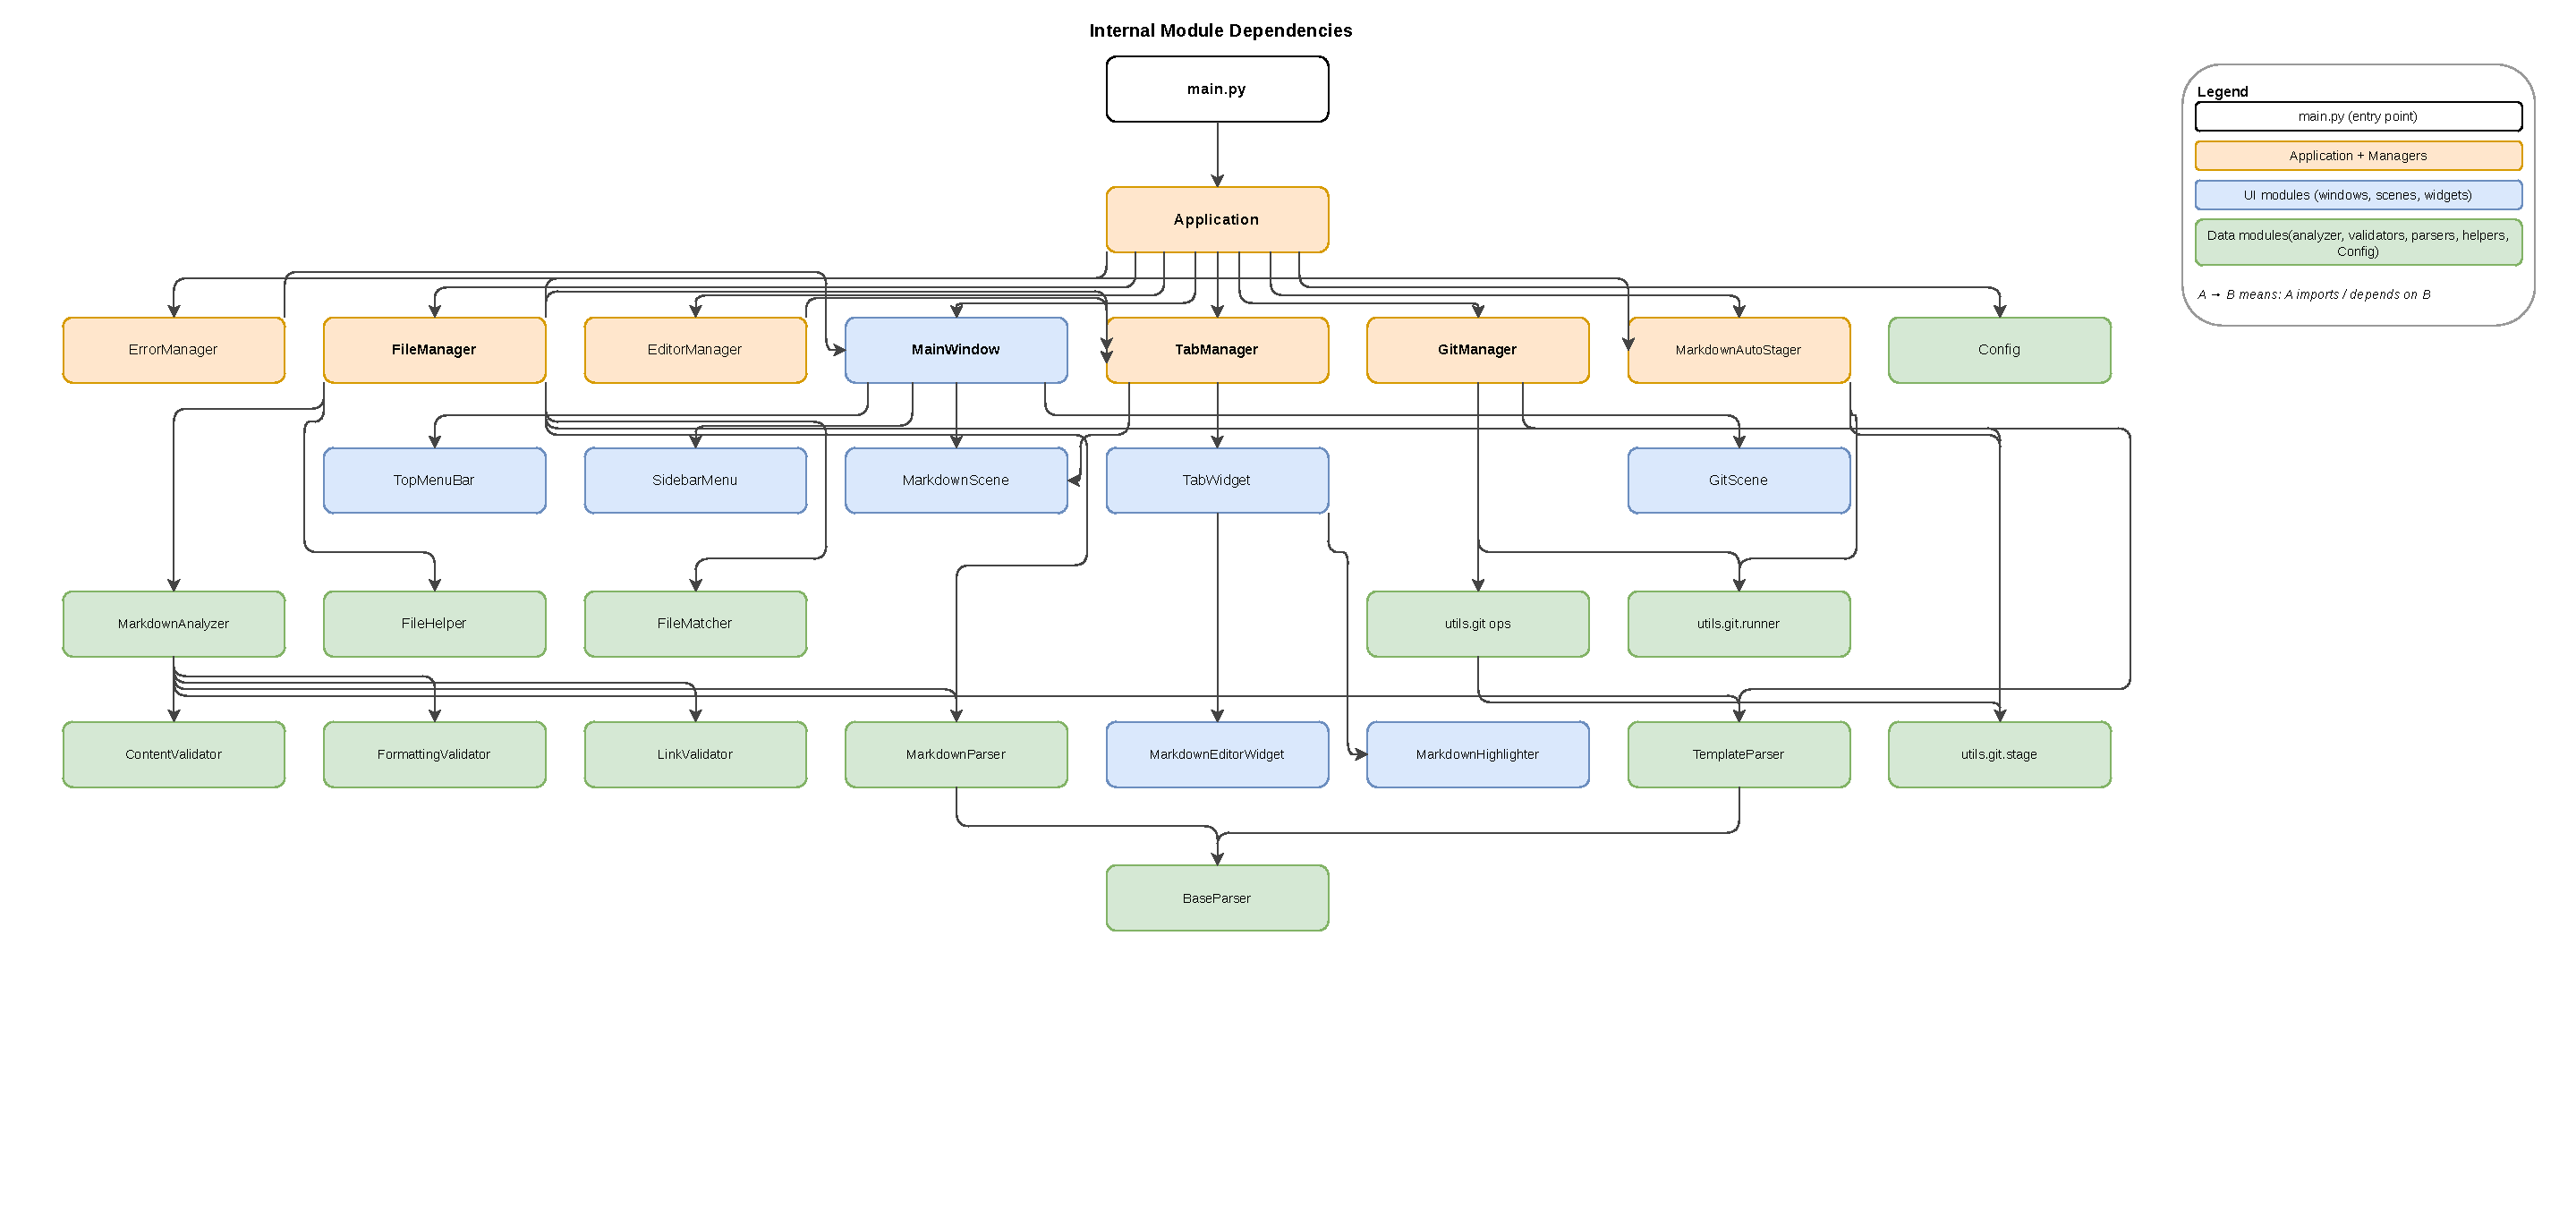
\includegraphics{images/dependency_diagram.pdf}}
    \caption{Dependencies of the main application modules (imports and layers between the entry point, 
    application, managers, user interface, and helper libraries).}
    \label{fig:diagram-dependency}
\end{figure}

\begin{figure}[H]
    \centering
    \adjustbox{max width=\textwidth,max height=0.93\textheight,center}{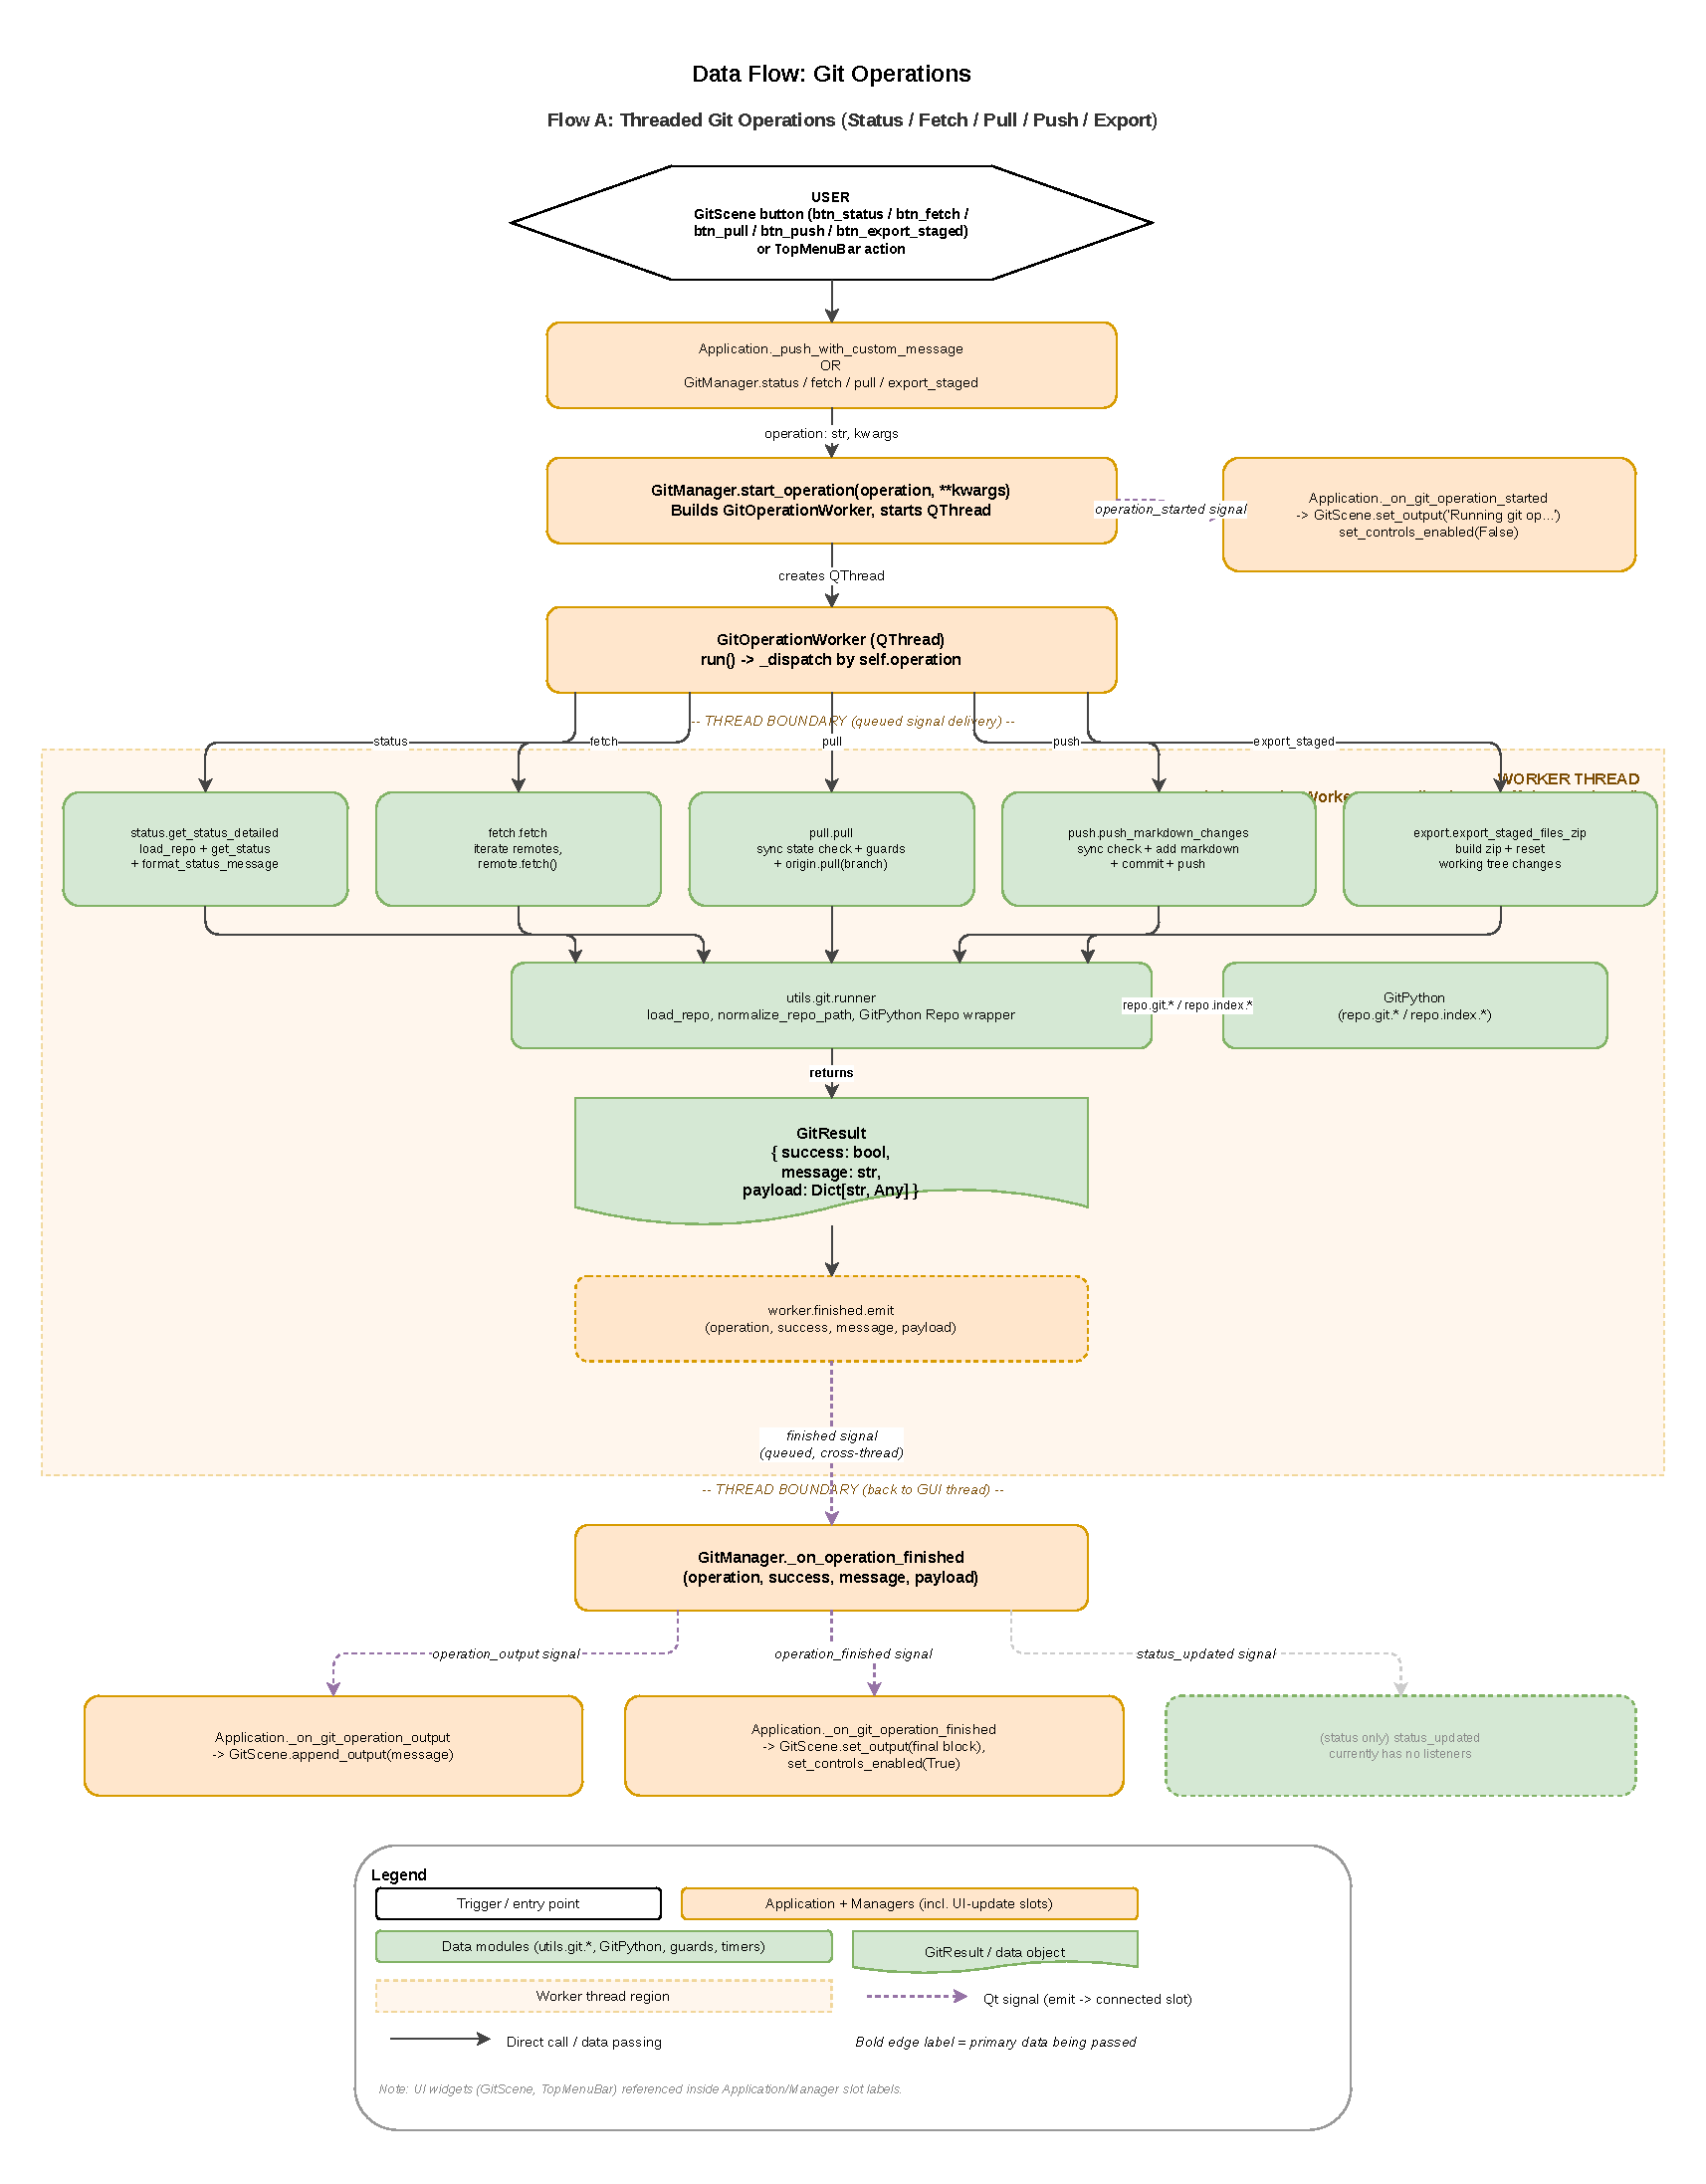
\includegraphics{images/dataflow_git_a.pdf}}
    \caption{Data flow during Git operations (Flow A): user action in Git Scene or menu,
     orchestration in \texttt{GitManager}, execution of commands in the \texttt{GitOperationWorker} thread using the \texttt{utils/git} package and GitPython, and feedback to the interface console.}
    \label{fig:dataflow-git-a}
\end{figure}

\begin{figure}[H]
    \centering
    \adjustbox{max width=\textwidth,max height=0.93\textheight,center}{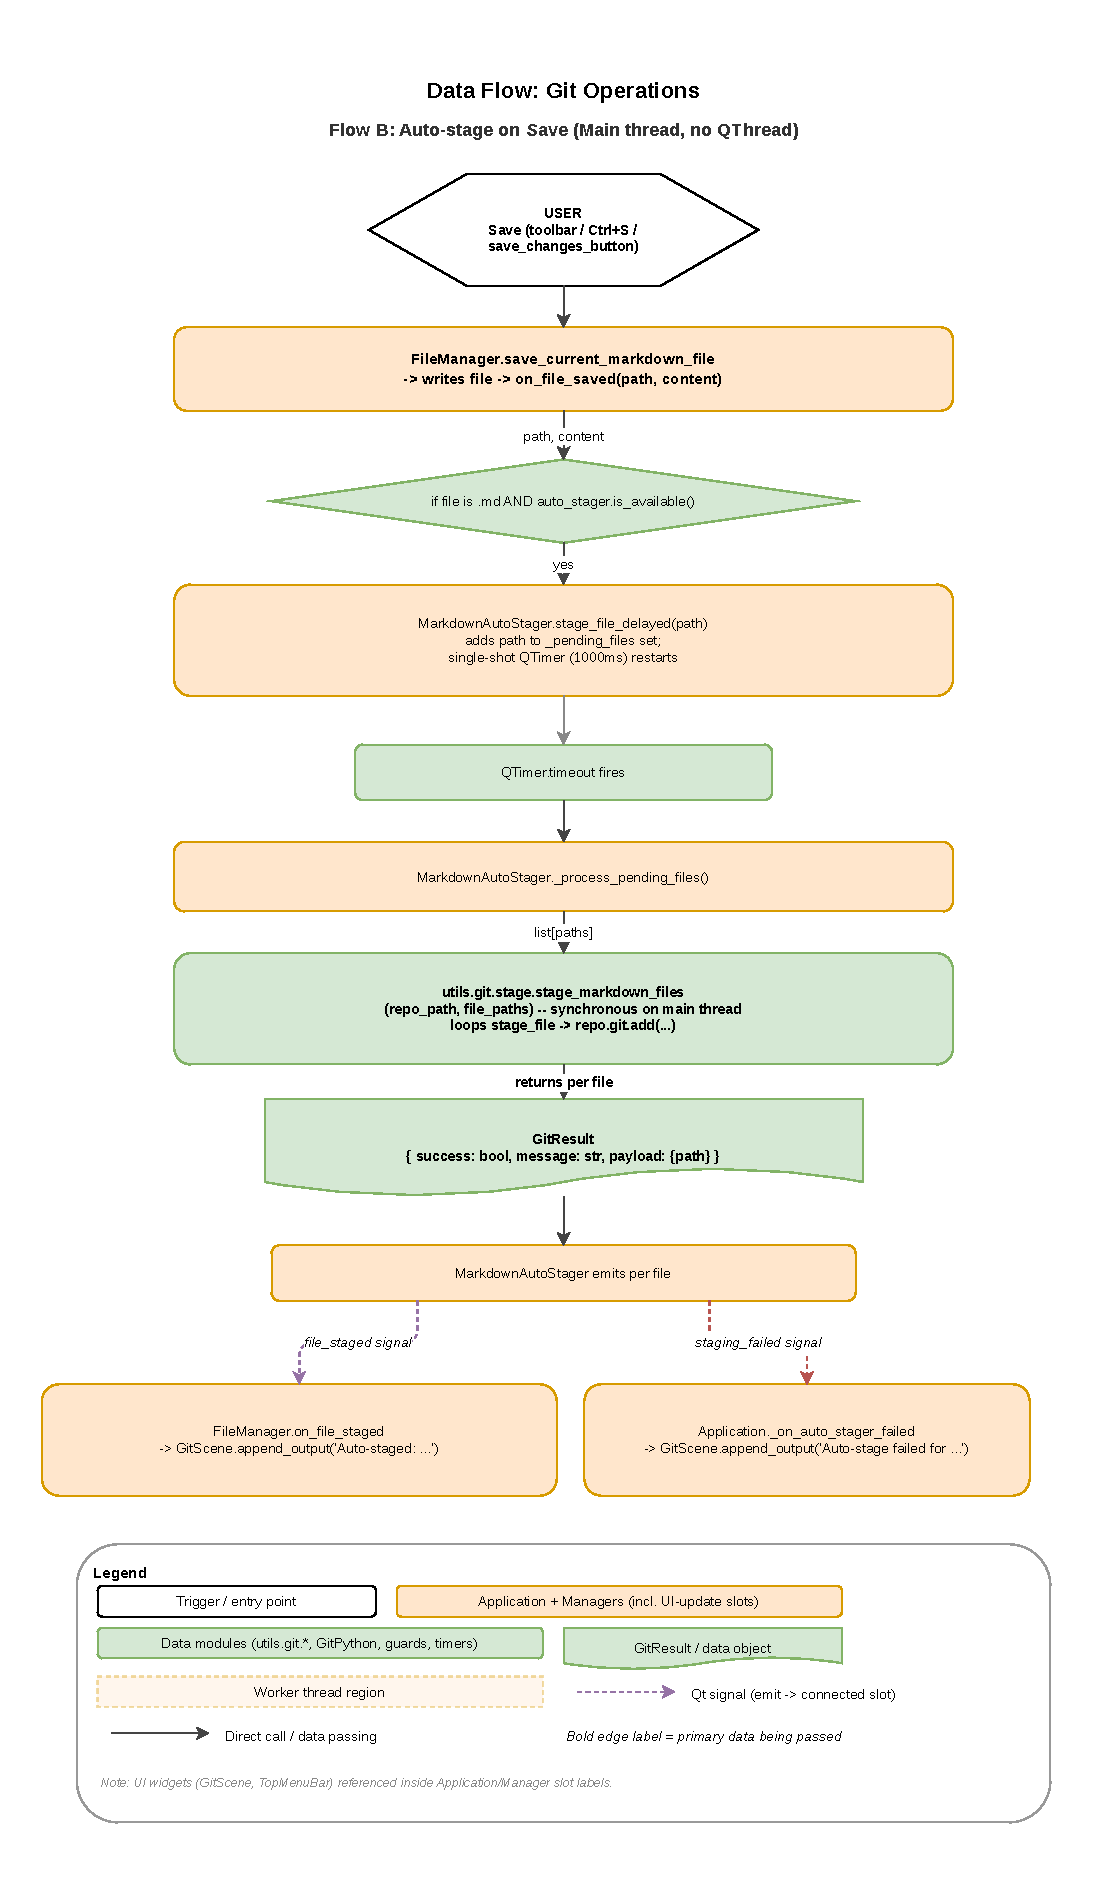
\includegraphics{images/dataflow_git_b.pdf}}
    \caption{Data flow during Git operations (Flow B): background automatic change staging 
    (Auto-stager) triggered after saving a file.}
    \label{fig:dataflow-git-b}
\end{figure}

\begin{figure}[H]
    \centering
    \adjustbox{max width=\textwidth,max height=0.93\textheight,center}{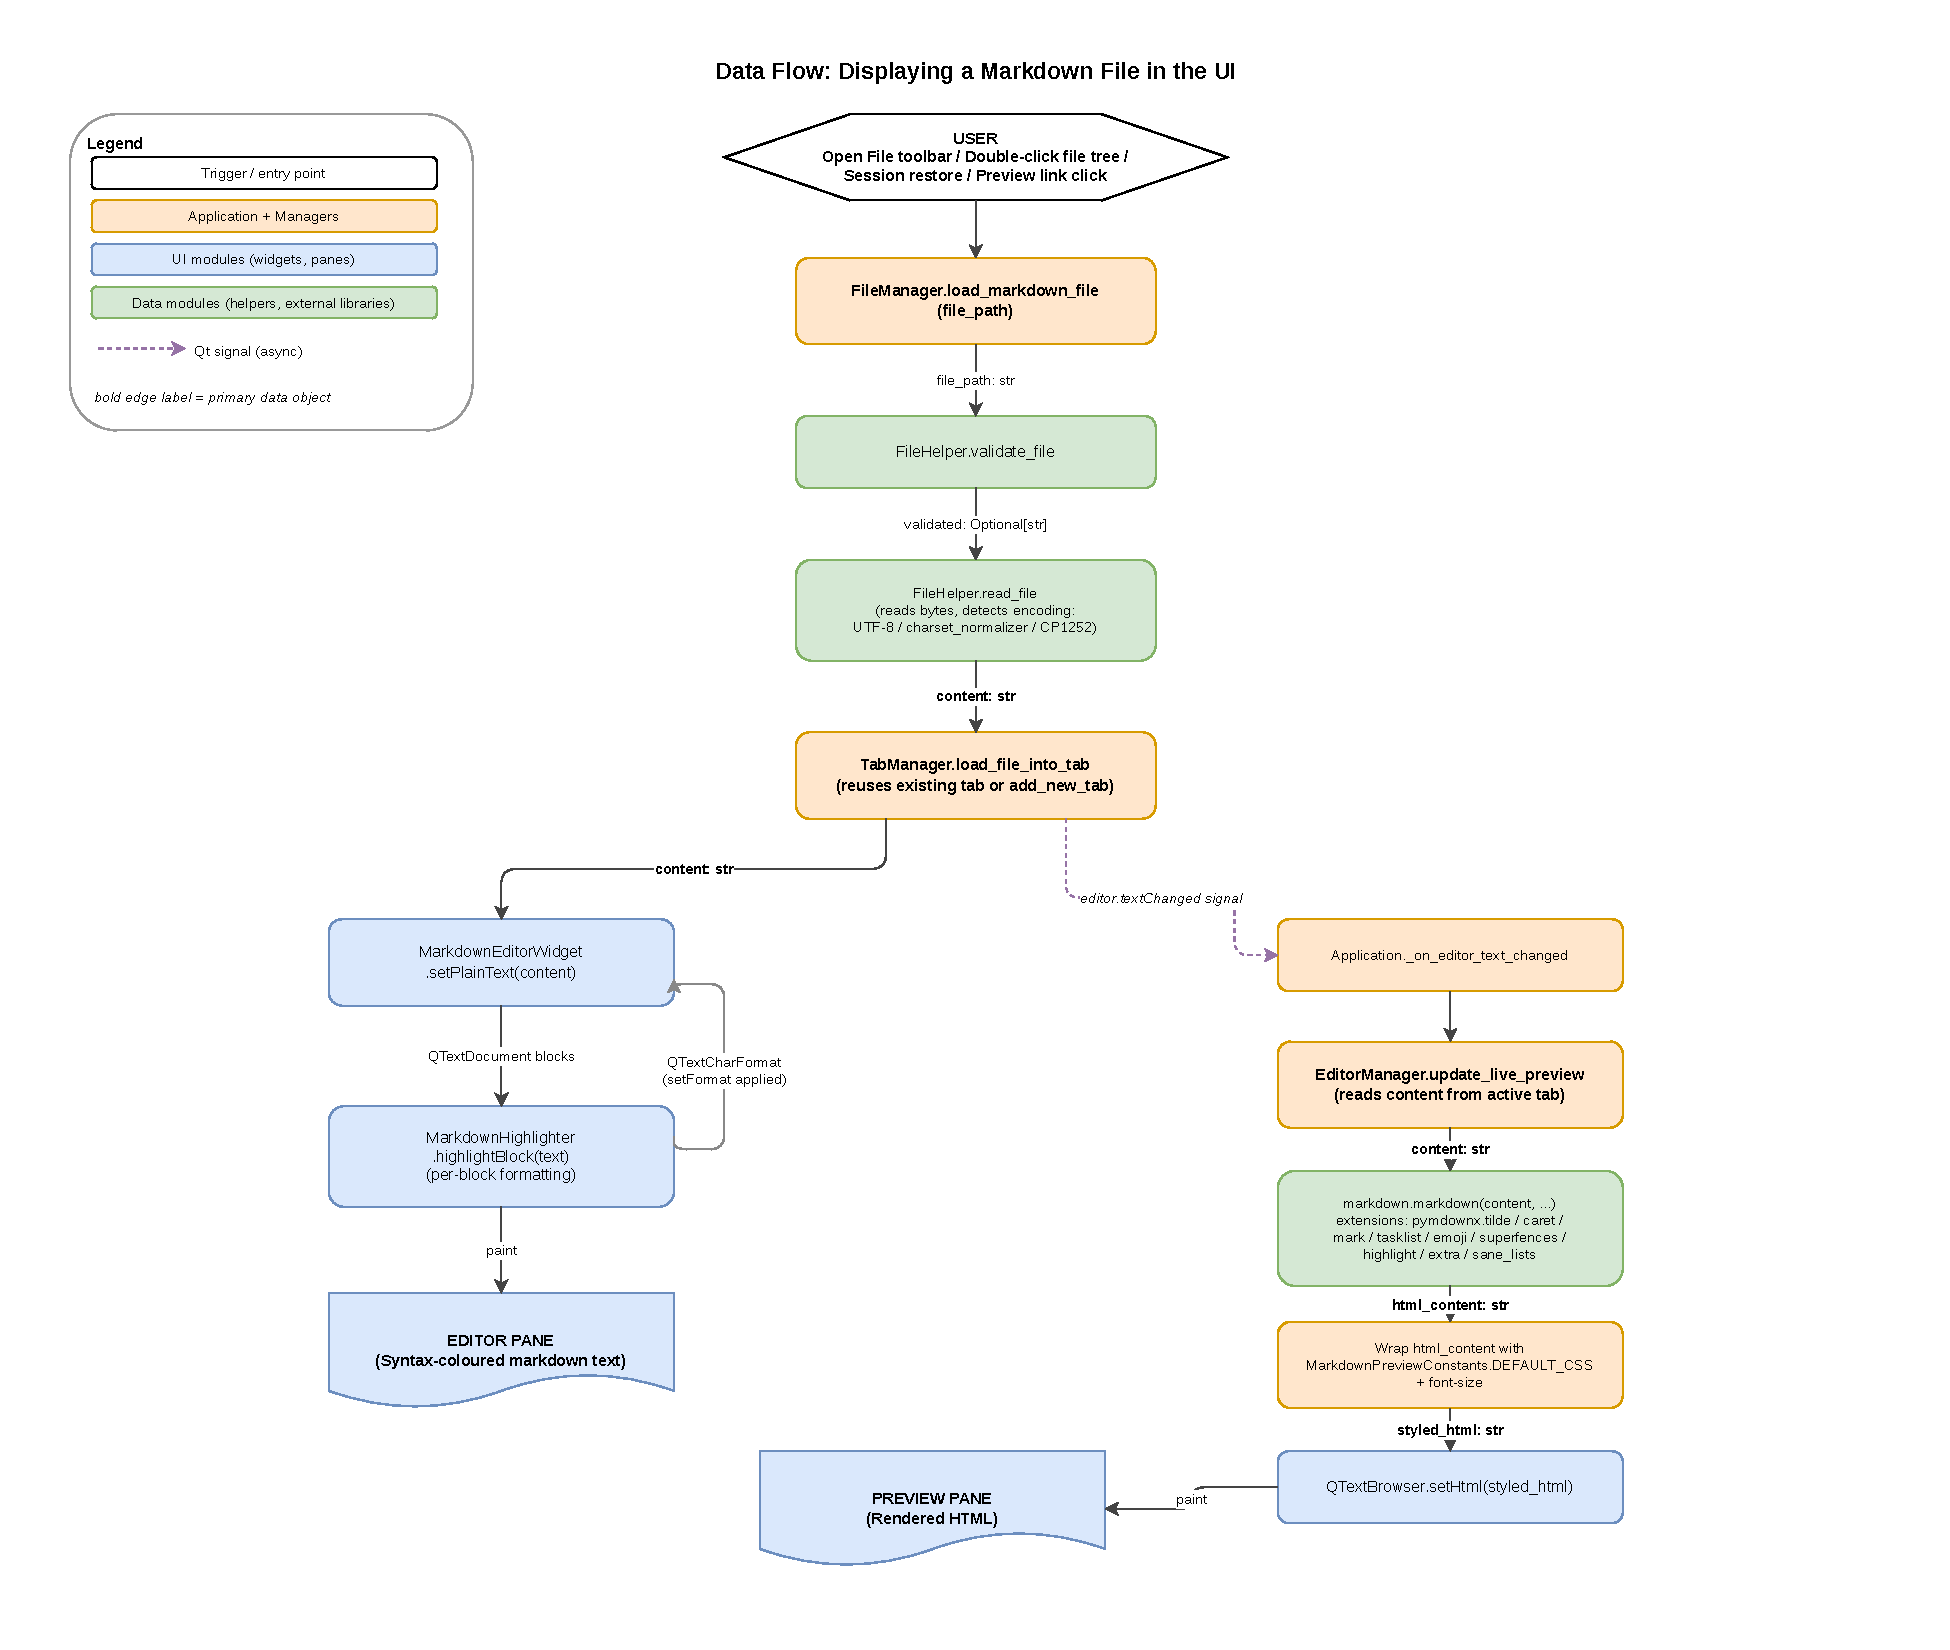
\includegraphics{images/dataflow_display.pdf}}
    \caption{Data flow during markdown file display: \texttt{FileManager} uses \texttt{FileHelper} for content validation and loading, \texttt{TabManager} handles tabs and the editor; the live preview is generated by converting markdown to HTML and rendering it in the preview widget.}
    \label{fig:dataflow-display}
\end{figure}

\begin{figure}[H]
    \centering
    \adjustbox{max width=\textwidth,max height=0.93\textheight,center}{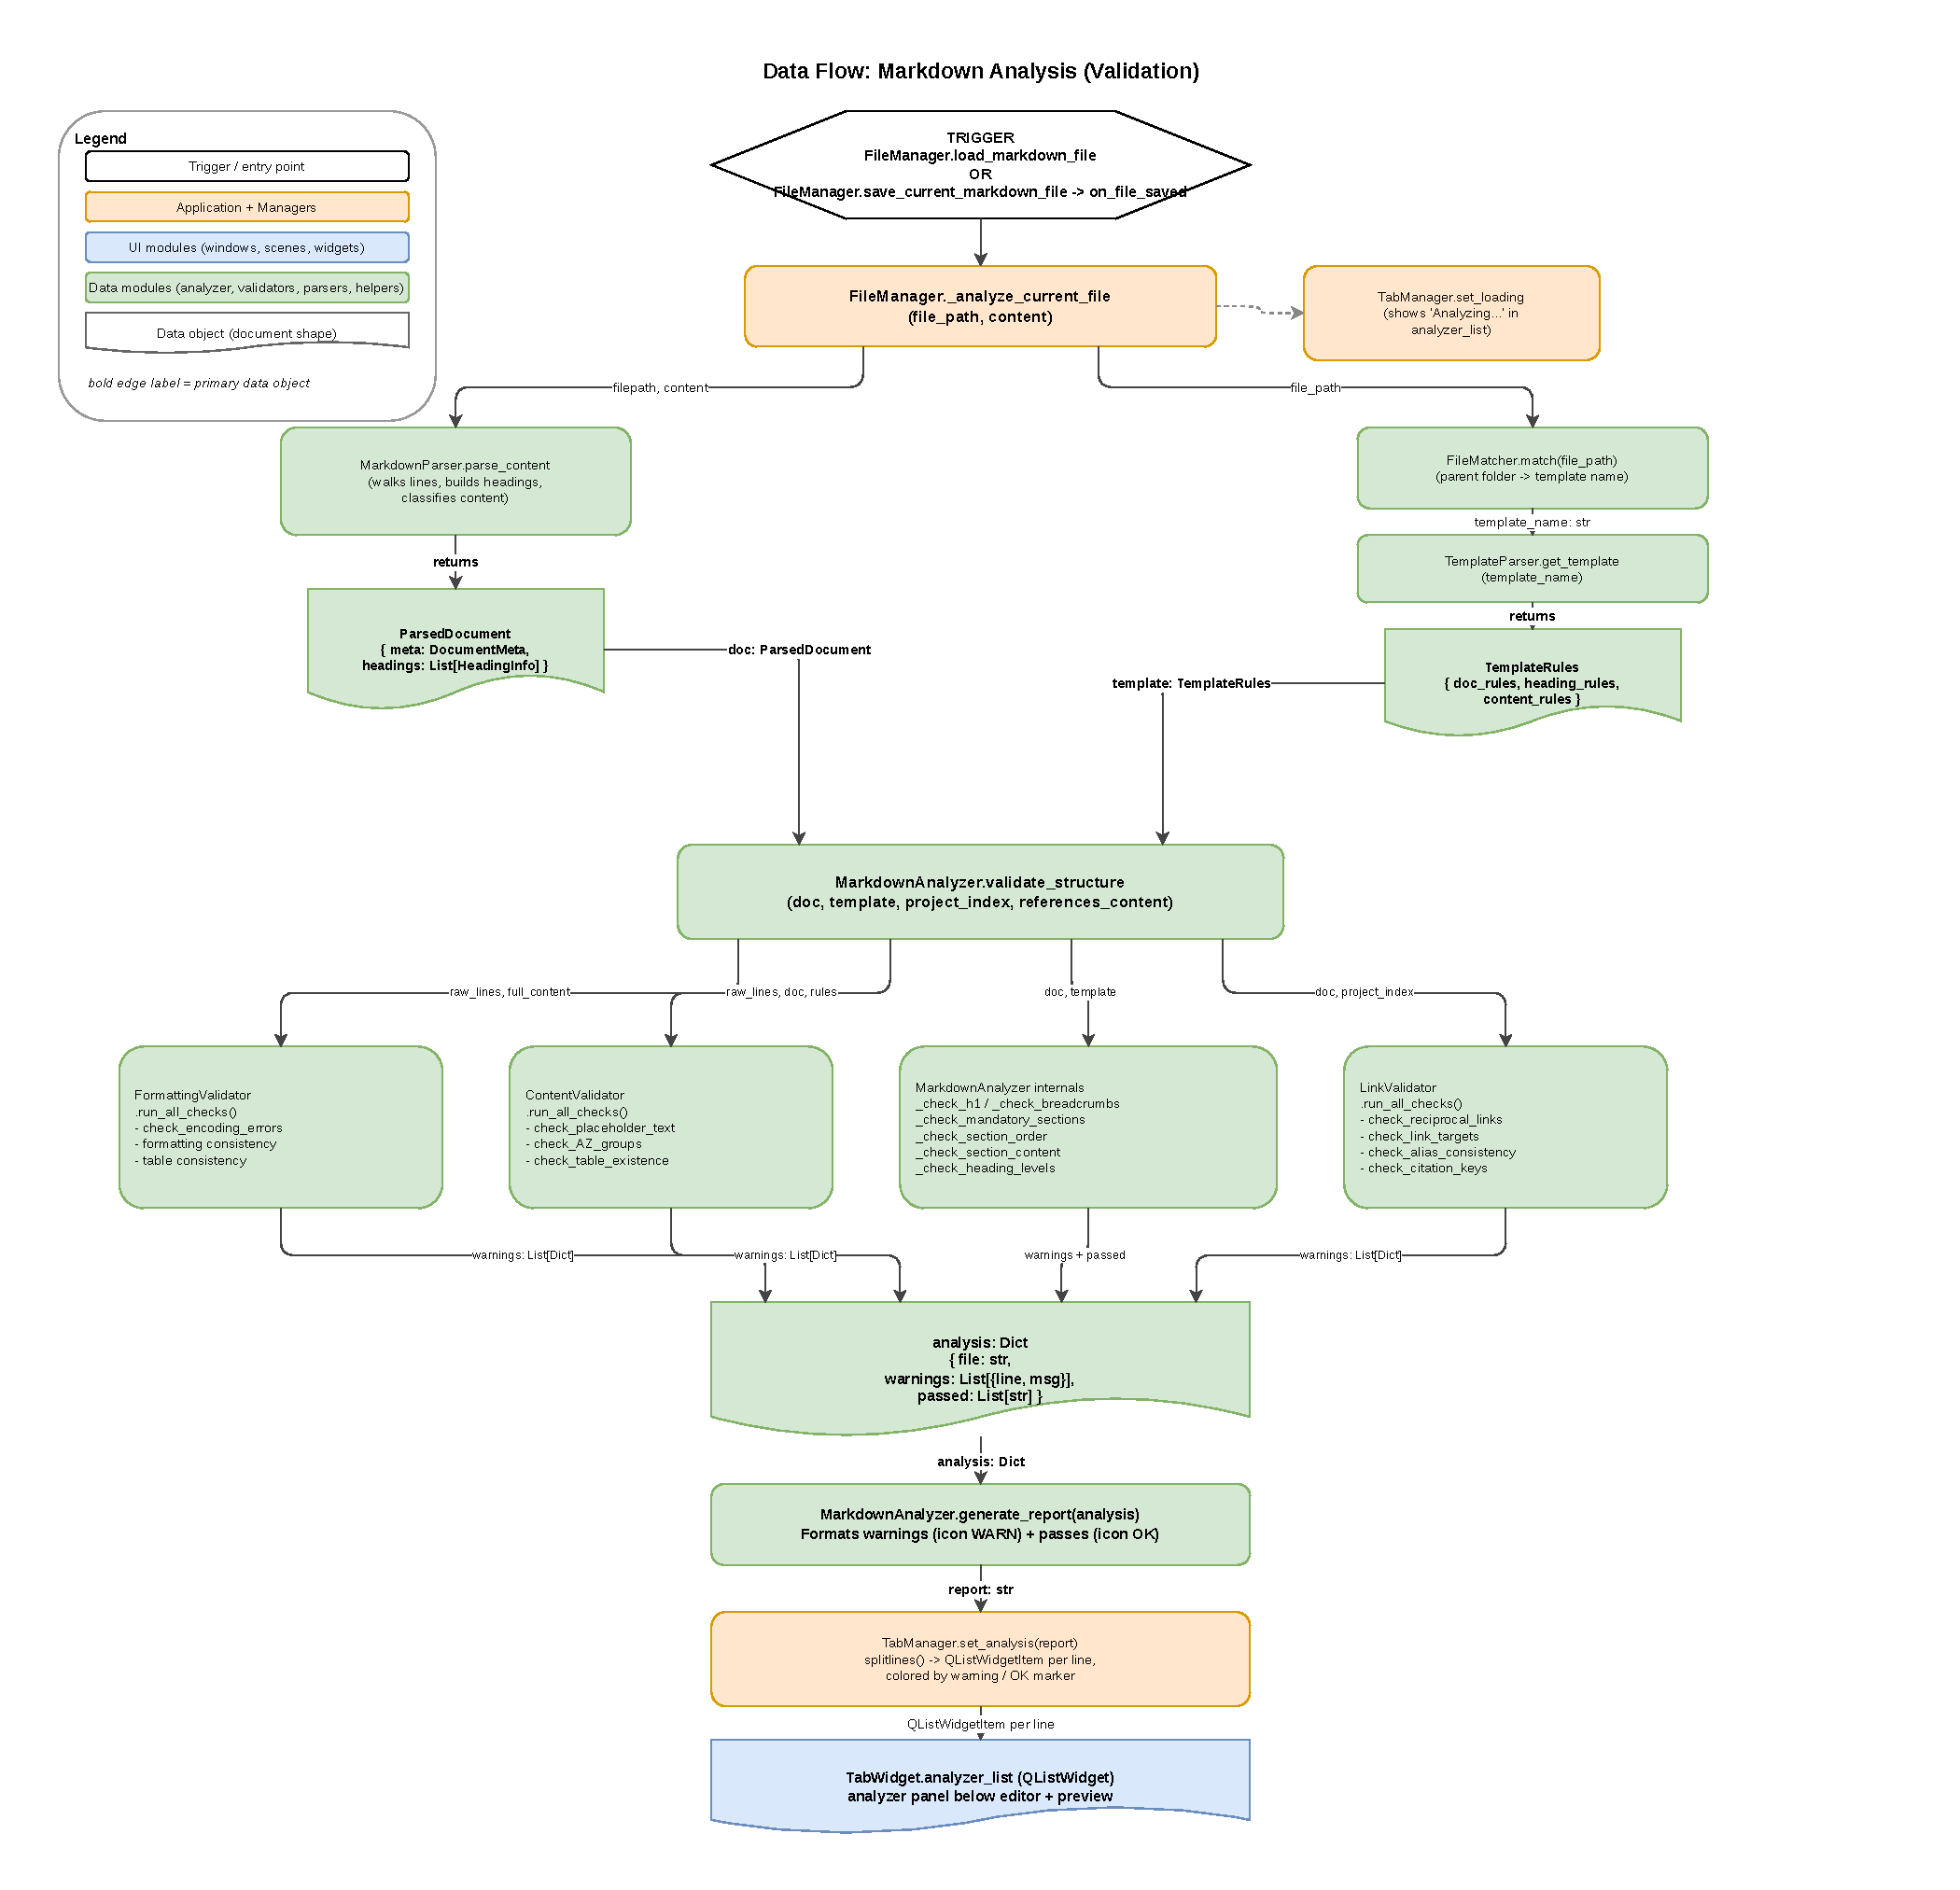
\includegraphics{images/dataflow_analysis.pdf}}
    \caption{Data flow during markdown structure analysis and validation upon loading or saving: from \texttt{FileManager} through document parsing, template selection, down to the validators and printing of results in the analyzer panel.}
    \label{fig:dataflow-analysis}
\end{figure}

\clearpage
\restoregeometry

\subsection{Test Scenarios}
\label{app:scenare}

This document contains the main functional tests for the application, focusing on the user interface, error handling, and Git integration.

\subsubsection*{1. Git Operations}

\textbf{Scenario 1.1: Execute Git Push with an entered commit message} \\
\textbf{Description:} Verify that the application executes a push when the user enters a commit message.
\begin{itemize}
    \item \textbf{GIVEN} the user is in the Git view (Git scene) and has staged changes.
    \item \textbf{AND} the text field for the commit message contains text.
    \item \textbf{WHEN} the user clicks the "Push" button.
    \item \textbf{THEN} the background Git push operation EXECUTES.
\end{itemize}

\textbf{Scenario 1.2: Prevent Git Push with an empty commit message} \\
\textbf{Description:} Verify that the application blocks a push if the user forgets to enter a commit message.
\begin{itemize}
    \item \textbf{GIVEN} the user is in the Git view (Git scene) and has staged changes.
    \item \textbf{AND} the text field for the commit message is completely empty (or contains only spaces).
    \item \textbf{WHEN} the user clicks the "Push" button.
    \item \textbf{THEN} a critical dialog appears with the title "Missing Commit Message".
    \item \textbf{AND} the background Git push operation DOES NOT EXECUTE.
\end{itemize}

\textbf{Scenario 1.3: Export changed files} \\
\textbf{Description:} Verify that the user successfully exports changed files from the working directory.
\begin{itemize}
    \item \textbf{GIVEN} the user is in the Git view.
    \item \textbf{WHEN} the user clicks the "Export Staged" button.
    \item \textbf{THEN} a warning dialog appears with the title "Warning: Potential Data Loss".
    \item \textbf{WHEN} the user clicks "Yes".
    \item \textbf{THEN} the dialog closes and the export operation executes.
\end{itemize}

\textbf{Scenario 1.4: Prevent unintended data loss during Git Export} \\
\textbf{Description:} Verify that the user is warned prior to exporting, as this action clears the working directory.
\begin{itemize}
    \item \textbf{GIVEN} the user is in the Git view.
    \item \textbf{WHEN} the user clicks the "Export Staged" button.
    \item \textbf{THEN} a warning dialog appears with the title "Warning: Potential Data Loss".
    \item \textbf{WHEN} the user clicks "No".
    \item \textbf{THEN} the dialog closes and the export operation is canceled.
\end{itemize}

\subsubsection*{2. Application Exit and Tab Management}

\textbf{Scenario 2.1: Closing the application with unsaved tabs (Cancel)} \\
\textbf{Description:} Verify that the user can abort closing the application if there is unsaved work.
\begin{itemize}
    \item \textbf{GIVEN} the application is open and contains at least one unsaved tab (indicated by an asterisk * in the tab name).
    \item \textbf{WHEN} the user clicks the system button to close the window ('X').
    \item \textbf{THEN} a warning dialog appears prompting to Save, Discard, or Cancel.
    \item \textbf{WHEN} the user clicks "Cancel".
    \item \textbf{THEN} the dialog closes and the application remains open.
\end{itemize}

\textbf{Scenario 2.2: Saving unsaved tabs when closing the application} \\
\textbf{Description:} Verify that the user can successfully save their work during the application exit process.
\begin{itemize}
    \item \textbf{GIVEN} the application is open with an unsaved tab.
    \item \textbf{WHEN} the user clicks the system button to close the window ('X').
    \item \textbf{AND} a warning dialog appears prompting to Save, Discard, or Cancel.
    \item \textbf{WHEN} the user clicks "Save".
    \item \textbf{THEN} the given file is saved.
    \item \textbf{AND} the application terminates.
\end{itemize}

\textbf{Scenario 2.3: Discarding changes when closing the application} \\
\textbf{Description:} Verify that the user can intentionally discard changes and force the application to close.
\begin{itemize}
    \item \textbf{GIVEN} the application is open with an unsaved tab.
    \item \textbf{WHEN} the user clicks the system button to close the window ('X').
    \item \textbf{AND} a warning dialog appears prompting to Save, Discard, or Cancel.
    \item \textbf{WHEN} the user clicks "Discard".
    \item \textbf{THEN} the unsaved changes are ignored and the application terminates.
\end{itemize}

\subsubsection*{3. File Explorer and Link Validation}

\textbf{Scenario 3.1: Safely handling invalid relative links} \\
\textbf{Description:} Verify that clicking a broken link in the live preview does not crash the application.
\begin{itemize}
    \item \textbf{GIVEN} the user is viewing a markdown file in the editor.
    \item \textbf{AND} the live preview panel is visible.
    \item \textbf{WHEN} the user clicks on a relative link in the preview that points to a non-existent file (e.g., \texttt{./missing\_document.md}).
    \item \textbf{THEN} a critical dialog appears with the title "Link Error".
    \item \textbf{AND} the application remains stable and active.
\end{itemize}

\textbf{Scenario 3.2: Safely handling external file deletion} \\
\textbf{Description:} Verify that the application starts up safely even if a previously opened file was deleted by the operating system.
\begin{itemize}
    \item \textbf{GIVEN} the user has the file \texttt{notes.md} open in a tab.
    \item \textbf{AND} the user closes the application.
    \item \textbf{WHEN} the user deletes the file \texttt{notes.md} using the file explorer in Windows/macOS.
    \item \textbf{AND} the user launches the application again.
    \item \textbf{THEN} the application starts successfully without crashing.
    \item \textbf{AND} the tab for \texttt{notes.md} either does not restore, or displays a clean, empty workspace without the opened tab.
\end{itemize}

\subsubsection*{4. Settings and State Persistence}

\textbf{Scenario 4.1: Remembering window dimensions and layout} \\
\textbf{Description:} Verify that the application restores its exact size and screen position.
\begin{itemize}
    \item \textbf{GIVEN} the application is running in windowed mode (not maximized).
    \item \textbf{WHEN} the user changes the window size to a specific dimension and moves it to a corner of the screen.
    \item \textbf{AND} the user closes and relaunches the application.
    \item \textbf{THEN} the application opens in the exact same position and size on the screen.
\end{itemize}

\textbf{Scenario 4.2: Restoring previously opened tabs} \\
\textbf{Description:} Verify that the user's workspace is preserved exactly as left.
\begin{itemize}
    \item \textbf{GIVEN} the user has exactly three different markdown files open in three tabs (\texttt{A.md}, \texttt{B.md}, \texttt{C.md}).
    \item \textbf{AND} tab \texttt{B.md} is currently active/focused.
    \item \textbf{WHEN} the user closes the application (saving any changes).
    \item \textbf{AND} the user relaunches the application.
    \item \textbf{THEN} all three tabs (\texttt{A.md}, \texttt{B.md}, \texttt{C.md}) are automatically restored.
    \item \textbf{AND} tab \texttt{B.md} is set as active/focused.
\end{itemize}

\textbf{Scenario 4.3: Restoring previously opened working directory} \\
\textbf{Description:} Verify that the opened working directory in the Explorer panel is preserved exactly as left.
\begin{itemize}
    \item \textbf{GIVEN} the user has a working directory open.
    \item \textbf{WHEN} the user closes the application.
    \item \textbf{AND} the user relaunches the application.
    \item \textbf{THEN} the given working directory is displayed in the Explorer panel.
\end{itemize}

\subsubsection*{5. Live Editor and Interface Toggles}

\textbf{Scenario 5.1: Rendering the live preview in real-time} \\
\textbf{Description:} Verify that the live preview reacts instantly to changes in the editor.
\begin{itemize}
    \item \textbf{GIVEN} the user has an open markdown file.
    \item \textbf{AND} the "Live Preview" checkbox is checked and the preview panel is visible.
    \item \textbf{WHEN} the user types \textit{\# New heading} into the text editor.
    \item \textbf{THEN} the live preview panel updates immediately and displays the formatted \textit{H1} HTML heading without needing to save the file.
\end{itemize}

\textbf{Scenario 5.2: Toggling UI panels (specifically "Analyzer")} \\
\textbf{Description:} Verify that the UI cleanly hides and restores panels.
\begin{itemize}
    \item \textbf{GIVEN} the user is in the main view with markdown.
    \item \textbf{WHEN} the user unchecks the "Analyzer" checkbox.
    \item \textbf{THEN} the analyzer list completely disappears from the layout, freeing up more screen space for the editor.
    \item \textbf{WHEN} the user checks the "Analyzer" box again.
    \item \textbf{THEN} the analyzer list reappears and retains its previous content.
\end{itemize}

\textbf{Scenario 5.3: Toggling UI panels (specifically "Live Preview")} \\
\textbf{Description:} Verify that the UI cleanly hides and restores panels.
\begin{itemize}
    \item \textbf{GIVEN} the user is in the main view with markdown.
    \item \textbf{WHEN} the user unchecks the "Live Preview" checkbox.
    \item \textbf{THEN} the live preview completely disappears from the layout, freeing up more screen space for the editor.
    \item \textbf{WHEN} the user checks the "Live Preview" box again.
    \item \textbf{THEN} the live preview reappears with updated visuals if the content in the markdown file changed.
\end{itemize}

\subsubsection*{6. Markdown Analyzer Core}

\textbf{Scenario 6.1: Flagging missing required headings} \\
\textbf{Description:} Verify that the analyzer detects template structure violations.
\begin{itemize}
    \item \textbf{GIVEN} the user has loaded a project directory containing a template (\texttt{template\_pattern.md}) that requires the heading \textit{\#\# Tasks}.
    \item \textbf{WHEN} the user opens a file matching this template category, but the heading \textit{\#\# Tasks} is missing from the file.
    \item \textbf{THEN} a specific warning/error appears in the Analyzer panel notifying of the missing required structure.
\end{itemize}

\textbf{Scenario 6.2: Analyzer clears errors after correction} \\
\textbf{Description:} Verify that the analyzer updates dynamically when the user fixes an error.
\begin{itemize}
    \item \textbf{GIVEN} the Analyzer panel currently displays a structural error (e.g., missing mandatory heading).
    \item \textbf{WHEN} the user adds the missing heading into the editor.
    \item \textbf{AND} the user clicks "Save Changes".
    \item \textbf{THEN} the error is removed from the Analyzer panel and a "Passed" or "OK" status is displayed.
\end{itemize}

\subsubsection*{7. File Explorer Integration}

\textbf{Scenario 7.1: Double-click opens a new tab} \\
\textbf{Description:} Verify that the explorer correctly opens new tabs.
\begin{itemize}
    \item \textbf{GIVEN} the user has a project folder open in the Explorer panel.
    \item \textbf{AND} the file \texttt{sample\_pattern.md} is NOT currently open in any tab.
    \item \textbf{WHEN} the user double-clicks \texttt{sample\_pattern.md} in the Explorer tree.
    \item \textbf{THEN} a new tab is created for \texttt{sample\_pattern.md}.
    \item \textbf{AND} the new tab becomes active (focused).
\end{itemize}

\textbf{Scenario 7.2: Double-click on an already open file focuses it} \\
\textbf{Description:} Verify that the explorer does not create duplicate tabs for the same file.
\begin{itemize}
    \item \textbf{GIVEN} the user has a project folder open in the Explorer panel.
    \item \textbf{AND} the file \texttt{sample\_pattern.md} is already open in Tab 1 (the tab has the same name as the file).
    \item \textbf{AND} the user is currently viewing Tab 2.
    \item \textbf{WHEN} the user double-clicks \texttt{sample\_pattern.md} in the Explorer tree.
    \item \textbf{THEN} the application DOES NOT CREATE a duplicate tab.
    \item \textbf{AND} the application immediately switches focus back to Tab 1.
\end{itemize}

\subsubsection*{8. Background Auto-Stager}

\textbf{Scenario 8.1: Saving a file triggers the auto-stager} \\
\textbf{Description:} Verify that the Git manager silently stages files in the background.
\begin{itemize}
    \item \textbf{GIVEN} the user has a tracked markdown file open in the editor.
    \item \textbf{AND} the Git repository has no uncommitted changes.
    \item \textbf{WHEN} the user makes a text edit and clicks "Save Changes".
    \item \textbf{THEN} the file is saved to disk.
    \item \textbf{AND} an output message is appended to the Git view console confirming the specific file was successfully staged (auto-staged) in the background.
\end{itemize}

\subsubsection*{9. Top Menu \& Shortcuts}

\textbf{Scenario 9.1: Opening files and folders via the File menu} \\
\textbf{Description:} Verify that menu items and opening shortcuts trigger the correct system dialogs.
\begin{itemize}
    \item \textbf{GIVEN} the application is running and active.
    \item \textbf{WHEN} the user selects \textit{File $\rightarrow$ Open File} in the top menu (or presses \textit{Ctrl+O}).
    \item \textbf{THEN} a system dialog opens for selecting an \texttt{.md} file.
    \item \textbf{WHEN} the user selects \textit{File $\rightarrow$ Open Folder} (or presses \textit{Ctrl+F}).
    \item \textbf{THEN} a system dialog opens for selecting a project directory.
\end{itemize}

\textbf{Scenario 9.2: Saving via keyboard shortcut} \\
\textbf{Description:} Verify that the save keyboard shortcut correctly saves the active tab.
\begin{itemize}
    \item \textbf{GIVEN} the user has an active tab with unsaved changes (indicated by *).
    \item \textbf{WHEN} the user selects \textit{File $\rightarrow$ Save File} (or presses \textit{Ctrl+S}).
    \item \textbf{THEN} the current file is saved to disk.
    \item \textbf{AND} the unsaved changes indicator disappears immediately.
\end{itemize}

\textbf{Scenario 9.3: Toggling panels via the File menu (Toggles)} \\
\textbf{Description:} Verify that the menu correctly synchronizes the state of UI panels.
\begin{itemize}
    \item \textbf{GIVEN} the user is in the main view (Markdown scene).
    \item \textbf{WHEN} the user selects \textit{File $\rightarrow$ Open Explorer} (or presses \textit{Ctrl+E}).
    \item \textbf{THEN} the file explorer sidebar hides (if it was visible) or shows (if it was hidden).
    \item \textbf{AND WHEN} the user presses \textit{Ctrl+P} (Live Preview) or \textit{Ctrl+A} (Analyzer).
    \item \textbf{THEN} the respective panels in the editor show or hide and their checkboxes update automatically.
\end{itemize}

\textbf{Scenario 9.4: Launching basic Git operations via the menu} \\
\textbf{Description:} Verify that keyboard shortcuts trigger background processes correctly.
\begin{itemize}
    \item \textbf{GIVEN} the user has a repository open.
    \item \textbf{WHEN} the user selects \textit{Git $\rightarrow$ Status} (or presses \textit{Ctrl+Shift+S}).
    \item \textbf{THEN} the operation starts.
    \item \textbf{AND} even if the user is not currently in the Git view (Git scene), they will see the result in the console upon switching to it.
    \item \textit{(Note: This test repeats analogously for Fetch / Ctrl+Shift+F and Pull / Ctrl+Shift+L)}.
\end{itemize}

\textbf{Scenario 9.5: Safeguards for critical Git actions via the menu} \\
\textbf{Description:} Verify that triggering risky actions via menu or shortcut does not bypass our safeguards (message validation and data loss warnings).
\begin{itemize}
    \item \textbf{GIVEN} the commit message text field is empty.
    \item \textbf{WHEN} the user presses \textit{Ctrl+Shift+P} (Push).
    \item \textbf{THEN} the operation stops and a "Missing Commit Message" error dialog pops up.
    \item \textbf{AND WHEN} the user presses \textit{Ctrl+Shift+E} (Export Staged).
    \item \textbf{THEN} a "Warning: Potential Data Loss" dialog pops up just as it would if the user clicked the physical button.
\end{itemize}

\end{document}